%!TEX root = proyecto.tex

\chapter{Diseño y resolución}

%\linespread{1.5}

\section{Paul Viola and Michael Jones} \label{haar-like}

En 2001, el reconocimiento facial tuvo su primera aparición en el campo de la visión artificial como aplicación en tiempo real. Este avance fue de la mano de Paul Viola y Michael Jones. Análogamente, el punto de partida del estudio de este TFG. Durante este apartado, se estudiará el funcionamiento del algoritmo \textit{Viola-Jones face detector}, ideado por estos dos investigadores y se realizará una implementación del mismo mediante \textit{Python} y \textit{OpenCV} para comprobar como se comporta en la situación actual.

\subsection*{Método de estudio}

El trabajo de los expertos fue presentado por parte de la Universidad de Cambridge mediante un \textit{paper} (ensayo de la investigación). Y se introduce como: 
\begin{quote}
	"This paper describes a machine learning approach for visual object detection which is capable of processing images extremely rapidly and achieving high detection rates" \cite{paulViola}
\end{quote}

Para poder lograr esta afirmación se basan en un procedimiento de trabajo en dos fases: entrenamiento y detección. Igualmente, Paul y Michael dividen el proyecto en tres ideas principales para poder lograr un detector que se pueda ejecutar en tiempo real. Y estas son: la imagen integral, Adaboost (algoritmo de Machine Learning) y un método llamado \textit{attentional cascade structure}. 

Con todos estos puntos combinados lograron ingeniar un prototipo capaz de detectar caras humanas con un \textit{frame rate} de 15 fps. Fue diseñado para la detección de caras frontales, haciéndose difícil para posiciones laterales o inclinadas.

Las imágenes que se toman para realizar la detección pasan por una transformación del espacio de color a \textit{grayscale}. Con el objeto de encontrar características en ellas, llamadas \textit{haar-like features}. Nombradas así por su inventor Alfred Haar en el siglo XIX. En este trabajo se hacen uso de tres tipos de haar-like features, que son las siguientes:

\begin{figure}[htp]
	\centering
	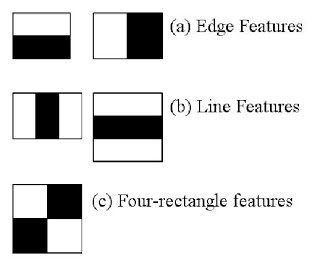
\includegraphics[width=5cm]{imagenes/haar-like.jpeg}
	\caption{Haar-like Features}
	\label{fig:haarLike}
\end{figure}

Las \textbf{\textit{Haar-like features}}, o también conocidas como \textit{Haar-wavelet} son una secuencia de funciones \textit{rescaled square-shaped}, siendo similares a las funciones de Fourier y con un comportamiento parecido a los \textit{Kernel} usados en las \textit{Redes Convolucionales} (matrices que consiguen extraer ciertas \textit{features} de la imagen de entrada). De manera que, las \textit{Haar Features} serán las características de la detección facial.

En un estudio ideal, los píxeles que forma el \textit{feature} tendrá una división clara entre píxeles de color blanco con los de color negro (Figura 4.1), pero en la realidad eso casi nunca se va a dar.

Más especificamente, las \textit{Haar-like features} están compuestas por valores escalares que representan la media de intensidades entre dos regiones rectangulares de la imagen. Estas capturan la intensidad del gradiente, la frecuencia espacial y las direcciones, mediante el cambio del tamaño, posición y forma de las regiones rectangulares basándose en la resolución que se define en el detector. \cite{haar-like}

Estas características van a ayudar al ordenador a entender lo que es la imagen estudiada. Van a ser utilizadas mediante \textit{Machine Learning} para detectar donde hay una cara o no, mediante un recorrido sobre toda la imagen. Esto conlleva una potencia de computación elevada. Para paliar este problema idearon el método de la \textit{Imagen Integral}.

La \textbf{\textit{Imagen Integral}} permite calcular sumatorios sobre subregiones de la imagen, de una forma casi instantánea. Además de ser muy útiles para las \textit{HAAR-like features}, también lo son en muchas otras aplicaciones.

Si se supone una imagen con unas dimensiones de $<w,h>$ (ancho y alto, respectivamente), la imagen integral que la representa tendrá unas dimensiones de $<w+1,h+1>$. La primera fila y columna de esta son ceros, mientras que el resto tendrán el valor de la suma de todos los píxeles que le preceden. \cite{integral-web} Ahora, para calcular la suma de los píxeles en una región especifica de la imagen, se toma la correspondiente en la imagen integral y se suma según la siguiente fórmula (siguiendo la numeración de la Figura \ref{fig:integral}):
\begin{center}
	$sum = L4 + L1 - (L2 + L3)$ 
\end{center}
\begin{figure}[htp]
	\centering
	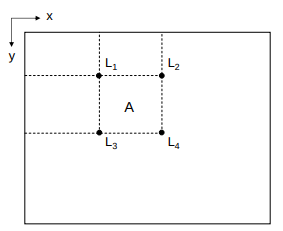
\includegraphics[width=5cm]{imagenes/integral.png}
	\caption{Funcionamiento de una \textit{Imagen Integral}}
	\label{fig:integral}
\end{figure}

Viola y Jones junta esta propuesta con los filtros \textit{Haar-like features}, y consiguen computar dichas características de manera constante y eficaz. \cite{integral}\\

% ---------------------------
%https://aishack.in/tutorials/integral-images-opencv/

%https://www.quora.com/How-integral-image-is-used-in-image-processing-and-how-improves-the-computation-time?share=1
%https://www.quora.com/What-are-the-must-read-papers-in-the-field-of-computer-vision-for-a-student-in-pursuing-research-in-the-field
% ---------------------------
%
% MACHINE LEARNING - ADABOOST
\newpage
Una vez estudiada la obtención de características y con un set de entrenamiento, solo queda seleccionar un método de \textit{machine learning} que permita crear una función de clasificación. Concretamente, se plantea el uso de una variante de \textbf{\textit{AdaBoost}}, que permite seleccionar un pequeño conjunto de características y poder entrenar un clasificador. 

Este algoritmo de aprendizaje esta basado en generar una predicción muy buena a partir de la combinación de predicciones peores y más débiles, donde cada uno de estas se corresponde con el \textit{threshold} de una de las características \textit{Haar-like}. La primera vez que aparece este algoritmo, de forma práctica, fue de la mano de \textit{Freund y Schapire} \cite{adaboost1}. Sin embargo, el usado por \textit{Viola y Jones} es una modificación de este.

La salida que genera el algoritmo \textbf{\textit{AdaBoost}} es un clasificador llamado \textit{Strong Classifier}, como se ha mencionado anteriormente, compuesto por combinaciones lineales de \textit{Weak Classifiers}. 

El procedimiento para encontrar \textit{Weak Classifiers} es ejecutar el algoritmo T iteraciones donde T es el número de clasificadores a encontrar. En cada iteración, el algoritmo busca el porcentaje de error entre todas las características y escoge la que menos porcentaje de error presente en dicha iteración. (Como se muestra en la \textit{Figura \ref{fig:ada1}}) \cite{adaboost2}

\begin{figure}[htp]
	\centering
	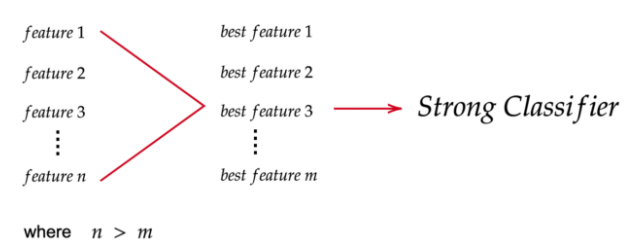
\includegraphics[width=10cm]{imagenes/ada1.png}
	\caption{Construcción del \textit{Strong Classifier}}
	\label{fig:ada1}
\end{figure}

Con estos clasificadores se procede a la construcción de una estructura en cascada para crear un \textit{Multi-stage Classifier}, que podrá realizar una detección rápida y buena. Por tanto, la estructura de cascada esta compuesta por varios estados de \textit{Strong Classifiers} generados por el algoritmo \textit{AdaBoost}. Donde el trabajo de cada estado será identificar si, dada una región de la imagen, no hay una cara o si hay la posibilidad de que la haya. \cite{adaboost1}

Si el resultado de uno de los estados es que no existe una cara en dicha región, esta se descarta directamente. Mientras que, si hay la posibilidad de que exista una, pasa al siguiente estado de la estructura. De tal forma que, cuantos más estados atraviese una región de la imagen, con más seguridad se podrá afirmar que existe una cara en ella. La estructura completa se refleja en la \textit{Figura \ref{fig:ada2}}.

\begin{figure}[htp]
	\centering
	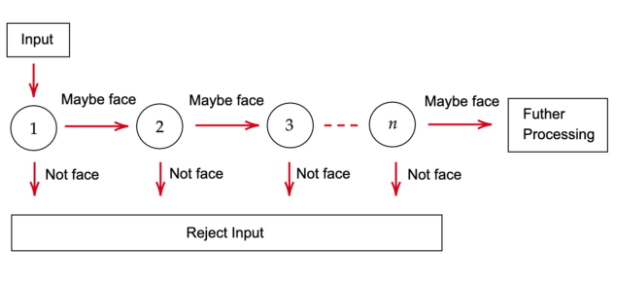
\includegraphics[width=10cm]{imagenes/ada2.png}
	\caption{Construcción del \textit{Multi-stage Classifier}}
	\label{fig:ada2}
\end{figure}

% VIDEO DE LOCOS: https://www.youtube.com/watch?v=uEJ71VlUmMQ&t=5s

\subsection*{Implementación y Experimentación}

El prototipo será implementado en \textit{Python}, con el uso de \textit{OpenCV}. Y, el objetivo es construir dos detectores de caras, donde el primero usará un modelo preentrenado de \textit{OpenCV} de caras frontales. Mientras que en el segundo, se intentará modificar el programa, para que mediante el uso de varios modelos preentrenados se pueda detectar una cara con una mascarilla.

La \textbf{implementación básica} hace uso de un modelo preentrenado cargado mediante una clase de \textit{OpenCV} llamada \textit{Cascade Classifier}. Esta representa la base de \textit{Machine Learning} explicado en el apartado anterior. Asimismo, \textit{OpenCV} también proporciona una serie de archivos \textit{xml} con diferente modelos preentrenados. En concreto, para este prototipo se hace uso del modelo por defecto, detector de caras frontal, como se muestra en la investigación de \textit{Viola y Jones}.

Finalmente, la detección se realiza, tras realizar una transformación del espacio de color a blanco y negro, mediante la función \textit{detectMultiScale} de la clase, creada anteriormente, \textit{Cascade Classifier}. Concretamente, su funcionalidad será encontrar caras dentro de las imágenes que vaya procesando.

[Explicacion del prototipo custom]

\textbf{OpenCV y Haar-like features + Machine Learning con PCA y SVM}
% Buscar como referencia para lo segundo HOG y SVM

Se implementa un identificador de caras conjunto a un modelo de \textit{Machine Learning} que identifica cuando una persona lleva o no mascarilla, mediante una toma de muestras anterior. Gracias a los modelos PCA y SVM, se puede crear un modelo para su identificador.
Lo malo: Solo funciona con los rostros/rostro que se toma como referencia para construir el modelo, igualmente pasa con el tipo de mascarilla (siendo la quirúrgica la que mejor funciona con este prototipo). Asimismo, su funcionamiento es de manera frontal y cercana, ya que si se coloca la cámara en la borde superior de una puerta o similar, el detector se pierde mucho y crea identificaciones falsa o no llega a reconocer nada.

Este procedimiento se podría llegar a usar con otra implementación, específicamente con HOG. 

[Resultados]
Bien, es un comienzo. Pero mal para un mercado amplio.

\newpage
\section{Facial Landmark}

Con el objetivo de ampliar la idea anterior, se plantea el uso de Facial Landmark, una tecnología que nos permite el reconocimiento de puntos de interés en las caras que se han detectado en la imagen. Sus pasos de ejecución son: detectar cara dentro de la imagen (En este caso, se usará \textit{Haar-like features}) y obtener dichos puntos de interés.

La implementación que se va a utilizar es la estudiada por \textit{Kazemi} y \textit{Sullivan} en 2014, con el paper \textit{One Millisecond Face Alignment with an Ensemble of Regression Trees} \cite{inproceedings}, y usado en el \textit{toolkit} \textit{Dlib}. Este método se centra en localizar las siguientes zonas faciales: boca, cejas, ojos, nariz y mentón, gracias al uso de un conjunto de árboles de regresión. Estos son entrenados mediante  un modelo formado por puntos de interés de un grupo de imágenes, etiquetados a mano y especificadas como coordenadas (x,y). 

\textit{Dlib} será el \textit{toolkit} (\textit{Open Source}) utilizado para la implementación de dicho método. Este contiene algoritmos de \textit{Machine Learning} y herramientas capaces de crear software complejo en \textit{C++} y \textit{Python} para resolver problemas reales. Sobre todo centrado en robótica, dispositivos embebidos, móviles y ordenadores de gran capacidad. \cite{dlib}

\subsection*{HOG - \textit{Histogram of Oriented Gradients}}

El primer paso en esta solución es encontrar una cara dentro de la imagen de entrada, y el encargado será el método HOG. El cual, sigue una idea similar al método de \textit{Haar-like}, ya que se basa en la detección de \textit{features} (características).

La idea teórica tras \textit{HOG} es encontrar la apariencia y forma de un objeto mediante la distribución de la intensidad de gradientes locales, gracias a que estos obtienen una magnitud mayor en las cercanías de bordes o esquinas. Mientras que la implementación, divide la imagen en pequeñas regiones (llamadas celdas) y se calculo un histograma de gradientes de 1 dimensión para cada uno de los píxeles de cada celda. Para un mejor estudio se normaliza el contraste de la imagen de entrada. \cite{hog} Con este procedimiento se obtiene un \textit{feature vector} a partir de la imagen de entrada, y la distribución resultante de los gradientes serán usados como las características. La implementación de HOG se podría dividir en 5 pasos generales \cite{hog2}:

\begin{enumerate}
	\item \textit{Pre-procesado}: Para una imagen de entrada de cualquier tamaño es tratada en regiones de ciertas escalas y analizadas en varias zonas de la imagen. La única restricción es que los tamaño de las regiones analizadas tienen una relación de aspecto fija.
	
	\item \textit{Cálculo de las imágenes de gradiente}: Para el calculo del histograma de gradientes es necesario realizar el calculo de los gradientes, tanto verticales como horizontales. Esto se puede obtener facilmente gracias al uso de \textit{Kernels} (filtros). Posteriormente, se busca la magnitud de las direcciones de dichos gradientes con el uso de la siguiente fórmula:
	
	\begin{figure}[htp]
		\centering
		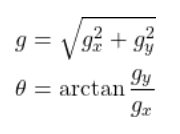
\includegraphics[width=3cm]{imagenes/HOGFormula.png}
		\caption{Fórmula \textit{HOG}}
		\label{fig:hogf}
	\end{figure}
	
	La fórmula esta implementada en \textit{OpenCV} mediante la función \textit{cartToPolar}. En este punto se puede obtener la imagen de los gradientes, eliminando toda la información no relevante de la imagen original, y se puede observar como en todos los pixeles el gradiente tomara una magnitud y una dirección. Si la imagen es RGB, los gradientes se evaluan sobre los tres canales de color, siendo la magnitud final el valor mayor entre los tres canales.
	
	\item \textit{Calculo de los histogramas de gradientes en celdas (8x8)}: La imagen se divide en celdas y se calculan los histogramas para cada una de ellas. Por ejemplo, si la celda es de tamaño 8x8, esta contendrá 192 píxeles (8x8x3), donde el gradiente tiene dos valores, descritos anteriormente (magnitud y dirección), por cada uno de los píxeles, lo que añade 128 valores (8x8x2). Esto facilita la representación de las regiones mediante el uso de un histograma, ademas mejora la influencia al ruido. El tamaño de la celda vendrá definida dependiendo de la escala de características (\textit{features}) que se estén buscando.
	
	\item \textit{Normalización de bloques (16x16)}: Una vez creado el histograma, hay que tener en cuenta que la imagen es sensible al brillo que tenga. Por ejemplo, si el brillo de la imagen se divide en dos, la magnitud del gradiente también lo hará. De igual forma, si el brillo se multiplica por dos, el gradiente ídem. Pero, se busca un descriptor que sea independiente a esto, por lo que se normaliza el histograma para que no se vea afectado por los cambios de luz/brillo.	Disponiendo de celdas de 8x8, un bloque de 16x16 posee cuatro histogramas que pueden ser condensados en un unico vector normalizado.
	
	\item \textit{Calculo del vector de HOG}: El último paso es concatenar los vectores normalizados obtenidos en uno global.

\end{enumerate}

Este procedimiento se repite varias veces sobre imagenes distintas y se introduce en un modelo \textit{Machine Learning} del tipo SVM Linear, con el objetivo de obtener un detector de caras. En el caso de \textit{Dlib}, posee un modelo preentrenado.


\subsection*{Sullivan Paper}

El \textit{paper} de Kazemi y Sullivan presenta la implementación usada en el \textit{toolkit Dlib} del algoritmo que estima de forma precisa y eficiente los puntos de interés faciales. Esta basado en \textit{gradient boosting} para el aprendizaje de un conjunto de arboles de regresión (\textit{ensemble of regression trees}), que será el encargado de la predicción de los puntos de interés.\cite{faceLandmark} 

Este método fue uno de los primeros que mejoro el rendimiento, a diferencia con los métodos anteriores, gracias a la detección de componentes esenciales para el \textit{face aligment} y procesarlos para introducirlos en funciones de regresión en cascada. Cada una de estas funciones estima, de forma eficiente, la forma facial desde una estimación inicial y obtiene un conjunto de píxeles indexados a dicha estimación. En concreto, \textit{Dlib} estimará un total de 68 píxeles indexados (Figura \ref{fig:dlibPoints}), ya que sigue las anotaciones del \textit{dataset iBUG 300-W} \cite{ibug}, usado en los modelos pre-entrenados ofrecidos por \textit{Dlib}.

\begin{figure}[htp]
	\centering
	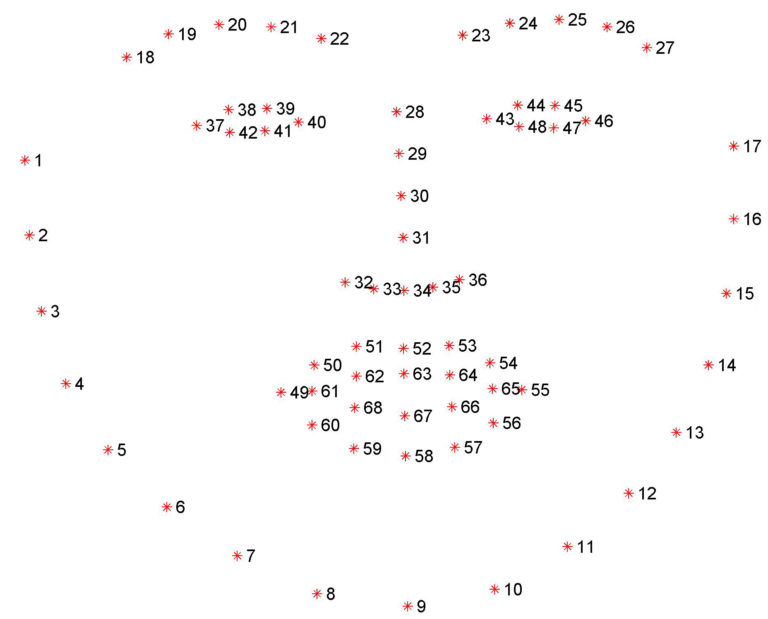
\includegraphics[width=8cm]{imagenes/facial_landmarks_68markup.jpg}
	\caption{68 coordenadas del \textit{facial landmark} con \textit{iBUG 300-W} \textit{dataset}}
	\label{fig:dlibPoints}
\end{figure}

Ademas, se introdujeron dos elementos clave a las funciones de aprendizaje de regresión. El primero gira en torno a la intensidad de los píxeles indexados con respecto a la estimación actual de la forma facial, ya que estos son muy influenciables por la deformación de la estimación de la forma y a los cambios de iluminación. El dilema que aparece es que necesitamos características confiables para obtener una predicción con precisión la forma y, por otro lado, necesitamos una estimación precisa de la forma para extraer características fiables. Para resolver este dilema se plantea el uso de un enfoque iterativo. La idea se basa en obtener una imagen transformada en un sistema de coordenadas normalizado basado en una estimación actual de la forma, y posteriormente extraer las características para predecir un vector de actualización para los parámetros de la forma. Este proceso suele repetirse varias veces.

El segundo elemento clave se trata de reducir la dificultad del proceso de inferencia/predicción. El objetivo es obtener una función capaz de estimar la forma que concuerde con la información de la imagen y el modelo. Pero el problema es que esta función es no convexa en varios valores locales. Para resolver esto se plantearon dos soluciones a lo largo del tiempo. El primero afirma que las predicciones estimadas en zonas lineales del subespacio mienten, y efectivamente ayuda a evitar este problema. Pero, posteriormente se descubrió la segunda solución, donde se asume que la función mienten en zonas lineales del subespacio y no es necesario realizar trabajo adicional. En el caso de este \textit{paper}, se implementa una solución donde se utilizan una combinación de ambas. Por lo que, cada regresor aprende mediante \textit{gradient boosting} conjuntamente a una función de perdida de error al cuadrado.

La entrada usada en el regresor, es seleccionada mediante \textit{gradient boosting} sobre un conjunto de píxeles dispersos, y la prioridad de probabilidad sobre la distancia entre pares de píxeles de entrada. Esto permite realizar un estudio sobre un mayor número de características relevante de forma eficiente. El resultado es una cascada de regresores que pueden localizar los puntos de referencia faciales cuando es inicializada con la media de la pose facial.

De forma más general, la investigación ofrece las siguiente contribuciones a las investigaciones de \textit{Face Landmark} anteriores:

\begin{enumerate}
	\item Un método de alineación que se basa en un conjunto de árboles de regresión que nos devuelve la forma facial mientras minimiza la función de error.
	\item Método que maneja la predicción de puntos que faltan o no están presentes en la imagen. Por ejemplo, rostros que estén medio ocultos. (Esto solamente se realizará si el modelo creado con HOG detecta dicha cara oculta).
	\item Resultados que demuestran que el método produce predicciones de alta calidad.
	\item El efecto de la cantidad de datos de entrenamiento.
\end{enumerate}

\subsection*{Prototipo}

Mediante \textit{OpenCV} y el \textit{ToolKit Dlib} se obtiene la implementación de ambas ideas, mediante modeles pre-entrenados.

\subsection*{Próximos pasos}

Con el objetivo de mejorar este prototipo se incorpora el \textit{Deep Learning}. En las últimas décadas, se ha convertido en uno de los métodos mas usados para la creación de aplicaciones de visión artificial. \cite{szeliski_2018}. Esta basado en las estructuras neuronales CNN (\textit{Convolutional Neural Network}), principales responsables de que un ordenador pueda procesar de forma sencilla una imagen. \textit{CNN} es una combinación entre capas neuronales y convolcionales, siendo estas últimas filtros con los que se obtendrán características de la imagen de entrada, los conocidos \textit{features}. La principal función del Deep Learning es clasificar, ya sea una imagen, un objeto o incluso varios objetos a la vez. Esto es gracias al uso de modelos, entrenados con miles de imágenes, que consiguen clasificar imágenes en varias categorías, por ejemplo \textit{MobileNet}. \cite{cnn}

En los siguientes apartados se probará implementar prototipos con el uso de Deep Learning con el objetivo de mejorar los resultado obtenidos hasta ahora. Se va a tratar con la API de Google llamada \textit{MediaPipe} y la tecnología de \textit{Transfer Learning} conjuntamente con \textit{TensorFlow}, para poder reentrenar modelos para nuestro objetivo, detectar mascarillas.

\newpage
\section{Mediapipe}

Mediapipe es una API \textit{open-source} creada por \textit{Google}, que ofrece servicios de \textit{Machine Learning} para vídeos y fuentes multimedia. Entre ellas, se encuentra un servicio llamado \textit{Face Mesh} que ofrece una solución que estima 468 puntos de interés de un rostro, que conforman una malla 3D en tiempo real. Este usa aceleración GPU conjuntamente con un modelo y el uso de una \textit{pipeline}.

La \textit{pipeline} que se utiliza en esta API consiste en dos modelos de \textit{Deep Learning} que trabajan al mismo tiempo. Su funcionalidad es realizar una detección a partir de una imagen de los puntos de interés sobre una cara y construir un modelo \textit{face landmark} 3D que aproxima la superficie de esta mediante regresión sobre dichos puntos. Esta tarea es facilitada si la cara, donde se tienen que detectar los puntos de interés, se encuentra recortada, haciendo así que el modelo se centre solamente en buscar los puntos, aumentando la precisión de la predicción. Asimismo, los recortes de las caras se puede generar a partir de las predicciones anteriores realizadas por el mismo modelo, y solamente es llamada la predicción nuevamente cuando no se consigue detectar la presencia de la cara.\cite{faceMesh}

Todo esto es implementado gracias al framework \textit{MediaPipe}, con la herramienta \textit{MediaPipe graph}. Arquitectura caracterizada por estar formada por componentes llamados \textit{Calculator}, nodos del grafo que tras la entrada de cero o más inputs generan cero o mas salidas. Todos estos nodos estan conectados mediante datos en forma de \textit{Streams}, donde cada uno representa un conjunto de datos-tiempo en \textit{Packets}. Por tanto, los \textit{calculators} y \textit{steams} definen el flujo de datos del \textit{Graph}. \cite{mediapipe}

El \textit{pipeline} puede ser definido mediante la adición/modificación de \textit{calculators} dentro del \textit{graph}. Especificamente, el pipeline que se utiliza en esta solución (\textit{FaceMesh}) esta formada por un \textit{graph} compuesto por un \textit{subgraph} de \textit{face landmark} (proveniente del modulo, ya implementado, de face landmark de Mediapipe), donde a su vez usa otro subgraph proveniente de face detection module para la detección de caras, y un \textit{face renderer subgraph} para mostrar el resultado. \cite{faceMesh} En concreto el \textit{graph} que se usa en esta implementación es el mostrado en la Figura \ref{fig:faceMesh}

\begin{figure}[htp]
	\centering
	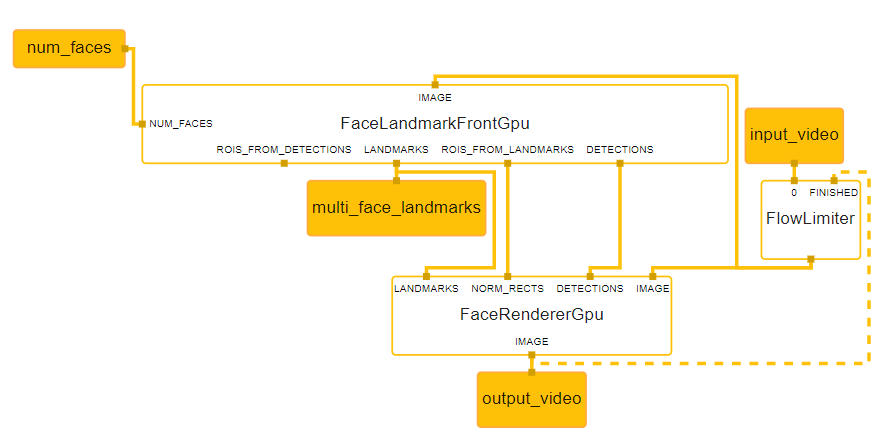
\includegraphics[width=15cm]{imagenes/faceMesh.png}
	\caption{MediaPipe Graph utilizado en FaceMesh}
	\label{fig:faceMesh}
\end{figure}

Por tanto, el procesamiento de una imagen en este modelo sigue dos pasos. El primero (1) toma la imagen de entrada, capturada por la cámara, es procesada por un detector de caras \textit{lightweigth}, llamado \textit{BlazeFace}, y produce unos rectángulos que definen el perímetro donde se encuentra la cara, conjuntamente con un par de puntos de interés superficiales (ojos, boca y nariz). Estos puntos se utilizarán para alinear la cara para el siguiente paso. Y el segundo (2), mediante el rectángulo obtenido en el paso anterior, se recorta la cara de la imagen inicial y es reescalado para utilizarse como entrada de la red neuronal que realiza la prediccion de la malla. (El tamaño de reescalado será entre 256x256 en un modelo completo, hasta 128x128 en el modelo más pequeño). Tras la predicción, se obtiene como salida un vector de coordenadas \textit{landmark 3D}, que serán mapeadas y dibujadas en la imagen original. \cite{faceMesh2}

Las coordenadas que se obtienen como salida estan compuestas por unas coordenadas x e y provenientes de localizaciones del plano 2D propio de la imagen. Mientras que, la coordenada z es interpretada como una profundidad relativa a un centro de masa que compone la malla de la cara.

Se utilizan dos modelos para el funcionamiento de \textit{FaceMesh}. El primero de ellos dedicado a la detección facial, llamado BlazeFace (mencionado anteriormente). Este es un modelo \textit{lightweight} creado para GPU móviles, llegando a una velocidad de procesamiento de entre 200 a 1000 fps en dispositivos móviles punteros. Es inspirado en los modelos \textit{MobileNet}, tanto la primera version como la segunda, provenientes del \textit{framework} SSD (\textit{Single Shot Multibox Detector}). Este modelo produce una salida compuesta por un rectángulo perimetral y 6 puntos de interés faciales. \cite{blazeface}

El segundo modelo, \textit{Face Landmark Model}, es generado mediante \textit{Transfer Learning} buscado una serie de objetivos: crear coordenadas 3D (mencionadas anteriormente) y conseguir mostrarlas en la imagen de salida de forma correcta. \cite{faceMesh} El \textit{Transfer Learning} es una técnica de \textit{Machine Learning} donde se puede hacer uso de un modelo preentrenado para personalizarlo y usarlo en una tarea determinada. Conviene destacar que un modelo entrenado es una red almacenada, entrenada previamente con un conjunto de datos con el objetivo de realizar una tarea de clasificación de imágenes a gran escala. \cite{transferLearning}

\textit{FaceMesh} propone una implementación mediante \textit{TensorFlow Lite} que dispone de dos formatos: CPU y GPU, que presentan un rendimiento en dispositivos moviles (\textit{Pixel3}, \textit{Pixel2} y \textit{iPhoneX}) muy fluido, impresionado sobre todo su funcionamiento sobre CPU. (Figura \ref{fig:faceMeshRen}) \cite{faceMesh3}

\begin{figure}[htp]
	\centering
	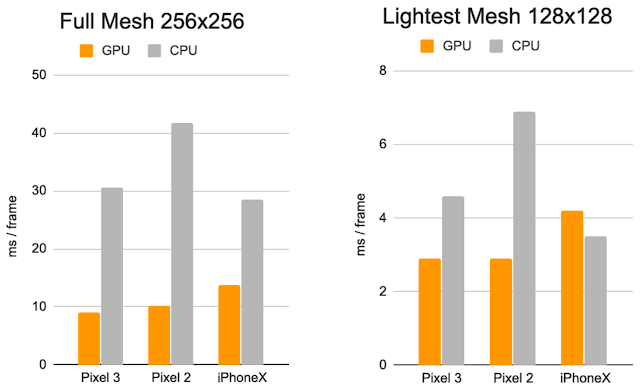
\includegraphics[width=10cm]{imagenes/rendFaceMesh.png}
	\caption{Rendimiento de FaceMesh sobre dispositivos móviles}
	\label{fig:faceMeshRen}
\end{figure}

\subsection*{SSD y MobileNet} \label{Mobilenet}

Explicar un poco.

\subsection*{Prototipo}

Uso de \textit{FaceMesh} del framework \textit{MediaPipe} y un detector basado en \textit{Haar-like features}, como el mencionado en el \textit{paper} de Viola \& Jones (\ref{haar-like}).

% Explicar mi prototipo

\newpage
\section{Tensorflow}

TensorFlow es una plataforma de \textit{Open Source} dedicada al aprendizaje automático. Permite compilar e implementar con facilidad aplicaciones con tecnología de AA. Esta se basa en tensores, matrices multidimensionales con un tipo uniforme, que si se está familiarizado con NumPy , los tensores son como \textit{np.arrays}. Con la característica de que nunca se puede actualizar el contenido de un tensor, solo crear uno nuevo. \cite{tensorflow}

Concretamente, se usarán los modelos y ejemplos de aprendizaje automático ofrecidos y entrenados mediante la API de alto nivel de Tensorflow para la implementación del último prototipo. Este recurso recibe el nombre de \textit{TensorFlow Model Garden} \cite{modelGarden}, y se trata de un repositorio con un diferentes implementaciones de modelos y soluciones modeladas para Tensorflow. Los modelos estan pre-entrenados mediante un dataset llamado \textit{COCO 2017} \cite{coco}.

%https://blog.tensorflow.org/2020/03/introducing-model-garden-for-tensorflow-2.html
De que dispone Model garden, Un poco mas de info de coco

COCO is a large-scale object detection, segmentation, and captioning dataset. COCO has several features.

Junto a esto se usa Transfer Learning. \textit{Explicar}

\subsection{Prototipo MobileNet}

Explicar Mobilenet y pruebas

\subsection{Prototipo RetinaNet}

Explicar RetinaNet y pruebas

\subsection{Prototipo YOLO}

Explicar YOLO y pruebas
%https://medium.com/analytics-vidhya/yolov3-custom-object-detection-with-transfer-learning-47186c8f166d
%https://github.com/hunglc007/tensorflow-yolov4-tflite

\newpage
\section{Comparación}